\chapter{Definições de base para uma improvisação de códigos}\label{cap:introducao}

Uma improvisação de códigos supõe ao menos um(a) artista-programador(a) capaz de reagir a um ou mais estímulos, e de codificá-lo(s) em caracteres textuais. Segundo Giovanni Mori \ver{cap:intro}, estes caracteres indicam como sons, imagens, cores, movimentos e tecidos são projetados, movimentados ou tramados  para quem vê o(a) artista-programador(a). Este momento que transita entre a elaboração da imaginação, e a codificação textual do que acontecerá, será o norteador deste documento. Ele é ilustrado no pequeno ciclo da \autoref{fig:bricolagem}:

\begin{figure}[!h]
  \centering
  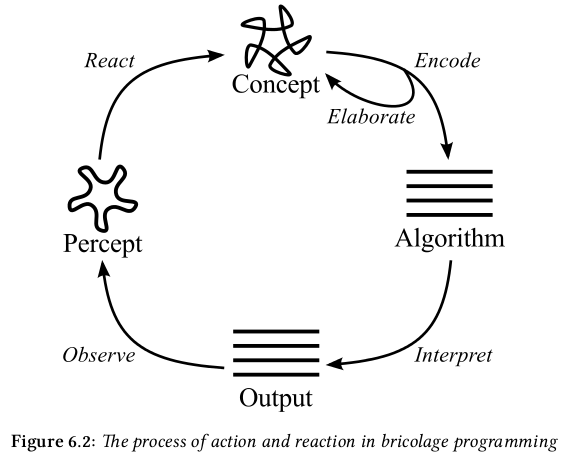
\includegraphics[scale=0.5]{./imagens/processo_criativo.png}
  \caption{O Processo de ação e reação no desenvolvimento de programas \emph{guiados por} bricolagem. Substituimos, ao longo deste trabalho, a palavra \emph{concept} (conceito) por \emph{proposição} para não confundirmos questões ontológicas. \textbf{Fonte}: \cite[p.~122]{McLean2011}, grifo nosso.}
  \label{fig:bricolagem}
\end{figure}

Começamos a investigação deste ciclo com um tipo específico de improvisação de códigos, o \emph{weavecoding} \ver{sec:weave}. Através de uma atividade  não-musical, buscamos ilustrar uma proposição e o código-fonte resultante. Costuramos este fio condutor com a Música Eletrônica para Dançar \ver{sec:slub}, e fechamos com uma proposição coreográfica \ver{sec:coreografia}.



\section{Tecendo códigos}\label{sec:weave}

O \emph{weavingcode} será definido conforme apresentamos o grupo \emph{Weaving codes}\disponivelem{http://kairotic.org/about/}, formado para  a \traducao{``(\ldots) investigação de padrões a partir das perspectivas de tecelagem e música, e através do desenvolvimento de uma linguagem de computador e código para descrever a construção de tecidos''}{We pursue these questions in the Weaving Codes- Coding Weaves project, by investigating patterns from the perspectives of weaving and music, and by developing a computer language and code for describing the construction of weaves}. É formado por membros das Universidades de Leeds, Nottingham Trent, Cambridge, Aberdeen, Copenhague; um museu (\emph{Albert Museum}), uma rede de laboratórios transdisciplinares (FoAM Kernow); o Centro Dinamarquês para Pesquisa Têxtil, e Escola Robert Schumman de Música e Mídia de  Düsseldorf.

Um de seus membros e um dos principais articuladores do \emph{live coding} inglês, Dave \citeonline{griffths_weave2_2015} descreve a seguinte proposição têxtil: com fios de tecido, são repetidas ações de dar a volta em pontos, pela frente, ou por trás do fio, afim de produzir uma figura geométrica. Estas ações são descritas em linguagem \emph{Scheme} a partir de quatro palavras-chave: \emph{repeat}, uma repetição de ações por contagem, ou laço iterativo (\emph{loop}); \emph{twist}, ou dar a volta em determinados pontos; \emph{weave-forward}, tecer o ponto alto; e \emph{weave-back}, tecer o ponto baixo. Do lado direito da imagem (ver p.~\pageref{fig:weaving}), é simbolizado o código compactado do tecido, ou as operações fundamentais para um determinado padrão têxtil. Do lado esquerdo, seu resultado, uma textura de losangos e zigue-zagues.  

\begin{example}{Um código-fonte que gera um tecido semelhante à \autoref{fig:weaving}.}
\label{ex:weaving}

\begin{minted}[fontsize=\footnotesize]{cl}
(twist 3 4 5 14 15 16)
(weave-forward 3)
(twist 4 15)
(weave-forward 1)
(twist 4 8 11 15)

(repeat 2
 (weave-back 4)
 (twist 8 11)
 (weave-forward 2)
 (twist 9 10)
 (weave-forward 2)
 (twist 9 10)
 (weave-back 2)
 (twist 9 10)
 (weave-back 2)
 (twist 8 11)
 (weave-forward 4))
\end{minted}
\end{example}

\begin{figure}[!h]
    \centering
    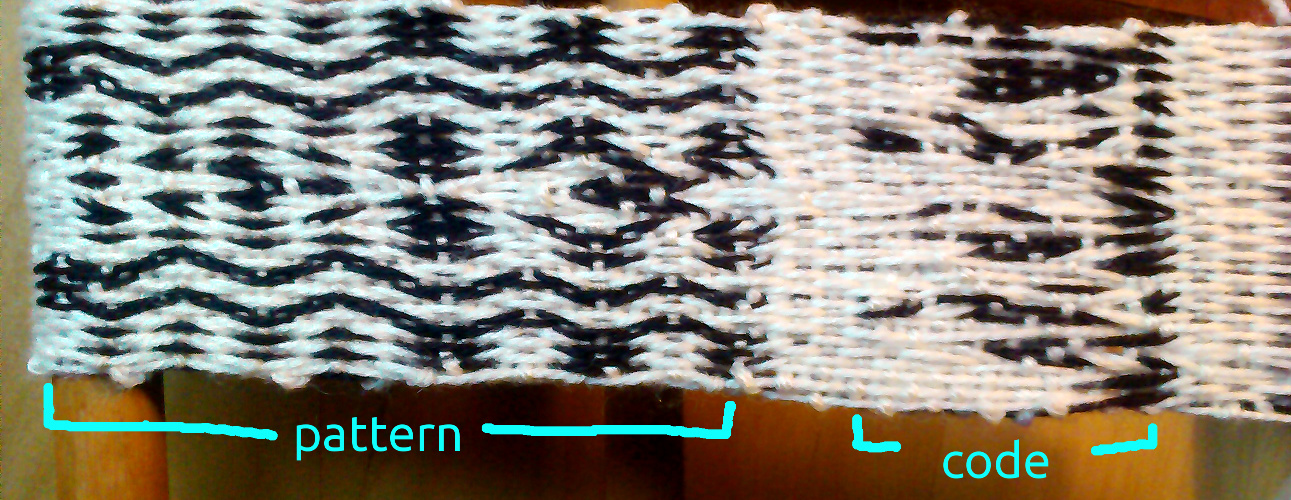
\includegraphics[scale=0.31]{imagens/weaving.jpg}
    \caption{Tecido resultante da prática \emph{Weaving code}. \textbf{Fonte}: \citeonline{griffths_weave2_2015}.}
  \label{fig:weaving}
\end{figure}

Esta experiência de \emph{participação social} \footnote{\cfcite{prospero_social_2015}} foi co-orientada por Griffths como uma \emph{sessão de improvisação}: programadores escrevem, enquanto observam e ouvem os resultados projetados por superfícies planas, caixas de som e máquinas de tear \ver{fig:weavecoding}. A tecelagem é programada por meio de um dispositivo tangível \ver{fig:weavecoding2} conectado a um computador portátil\footnote{Disponível em \url{https://www.raspberrypi.org/}}, uma matriz de botões acopláveis, desenvolvida por Ellen Harlizius-Klück (investigadora da história da matemática, filosofia e tecelagem da Grécia Antiga na Universidade de Copenhague\disponivelem{http://www.saumweberei.de/}) e Alex McLean (artista-programador de destaque). Imagens em movimento foram projetadas como capturas das atividades têxteis e processadas por Griffths. 

\begin{figure}[h]
  \centering
  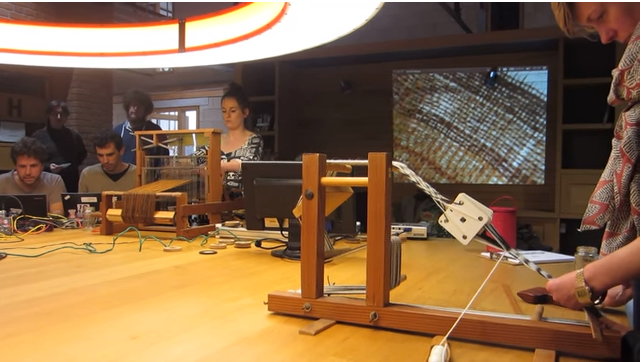
\includegraphics[scale=0.64]{imagens/weaving.png}
  \caption{Performance no Foam Kernow. \textbf{Fonte}: \citeonline{griffths_weave_2015}.}
  \label{fig:weavecoding}
\end{figure}

\begin{figure}[h]
  \centering
  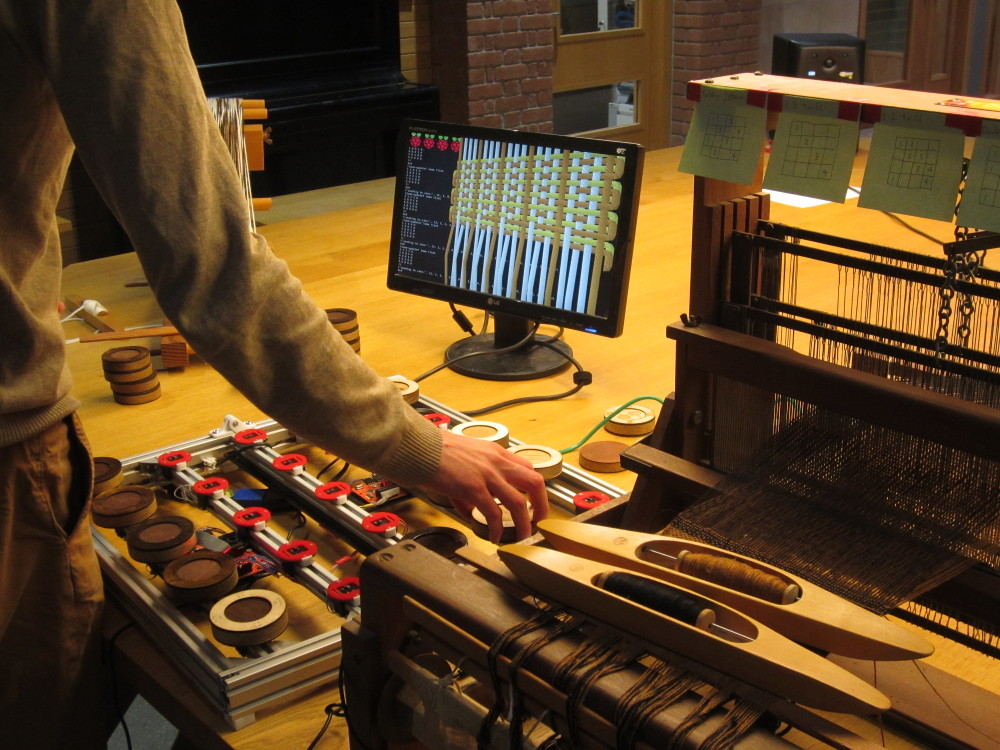
\includegraphics[scale=0.87]{imagens/weavecoding.jpg}
  \caption{ Alex McLean manipulando uma Matriz de botões para tecelagem, conectado a um Raspberry Pi. \textbf{Fonte}: \citeonline{griffths_weave_2015}.}
  \label{fig:weavecoding2}
\end{figure}

\begin{citacao}

\traducao{
Uma das ideias originais que tivemos foi combinar tecelagem e codificação em um cenário de performance, ambos como uma forma de tornar a codificação ao vivo mais inclusiva com a tecelagem, e ao mesmo tempo esclarecer os processos de pensamentos digitais envolvolvidos na tecelagem. (\ldots) Nossa audiência consistiu de pesquisadores de artesanato, biólogos antropológicos, arquitetos, designers de jogos e tecnólogos -- foi mais do que antecipamos! Alex e eu disponibilizamos alguns códigos de música do \emph{slub} para tecer, e minha parte favorita foi projetar a tecelagem ao vivo.
}{
One of the original ideas we had was to combine weaving and coding in a performance setting, to both provide a way to make livecoding more inclusive with weaving, and at the same time to highlight the digital thought processes involved in weaving. (\ldots) Our audience consisted of craft researchers, anthropological biologists, architects, game designers and technologists -- – so it all went on quite a lot longer than we anticipated! Alex and I provided some slub livecoded music to weave by, and my favourite part was the live weaving projection.
}
\end{citacao}

Esta descrição de Griffths possui uma documentação audiovisual \disponivelem{https://www.youtube.com/watch?v=XrnIVUp9QgM}.

\subsection{Slub}\label{sec:slub}

A parceria entre Griffths e McLean é essencial para entender o \emph{live coding} inglês. Ambos são membros da banda \emph{Slub}, que começou como uma colaboração entre Adrian Ward e Alex McLean. O grupo foca na atividade de programação para realização de uma Música Eletrônica para Dançar \footnote{\cfcite{hillegonda_dj_2013}}. 

Sua primeira reunião foi em 2001, no \emph{Paradiso club} em Amsterdã, durante o festival \emph{Sonic Arts}. Em 2005 Griffths se juntou ao duo durante o festival \emph{Sonar} em Barcelona, momento em que iniciaram um processo de \emph{gameficação} das performances, \cite[p.~138--140]{McLean2011}, e mais tarde, na inclusão de atividades têxteis. \citeonline[p.~139]{McLean2011} descreve um sistema \emph{Slub}, uma suíte de programas desenvolvidos para o fim específico de improvisar códigos:

\begin{citacao}
\traducao{Um sistema Slub antigo é descrito em detalhes por \citeonline{collins_generative_2003}. De maneira breve, ele apresentava um sintetizador, um antigo sistema de codificação ao vivo escrito por Ward, e uma série de programas geradores de batidas e linhas de baixo escritos por McLean. Embora o seu principal objetivo fosse musical, o$[$s membros do$]$ Slub gostavam de serem confrontados com o desafio de aceitação como programadores que fazem música. Para este fim, começaram a projetar suas telas de audiência com uma sobreposição conceitual, entre seu \emph{softwares} artesanais, e a música que  produziam com seu uso.}{An early Slub system is described in detail by \citeonline{collins_generative_2003}. In brief it featured a synthesiser and early live coding system written by Ward, and a Number of beat and bass-line generating programs by McLean. Although their primary aim was musical, Slub enjoyed beign faced with the challenge of beign accepted as programmers who make music. To this end they began projecting their screens audiences with the conceptual overlap between their and-crafted software and the music they produced using it.}
\end{citacao}

Em 2004, Ward e McLean focaram seus eforços no desenvolvimento de ambientes de improvisação de códigos, estruturados como editores de linguagens textuais ou visuais, e interfaces gráficas de usuário\footnote{\emph{Graphical User Interfaces} ou GUIs.}: \traducao{``O \emph{Slub} controlava sua música usando interfaces criadas por e para eles mesmos. Eles variam desde as $[$interfaces$]$ aparentemente convencionais para as abstratas, e das  gráficas para as inteiramente textuais''.}{Slub control their music using user interfaces created by and for themselves. These vary from the apparently conventional to the abstract, and from graphical to entirely textual.}
\cite[p.~323]{collins_generative_2003}:

\begin{citacao}
\traducao{Por detrás das interfaces \emph{slub} residem os processos 'composicionais' ou 'musicais' -- muitos pedaços de códigos separados, escritos como exploração de ideias musicais. Cada pedaço de código descreve um experimento em áreas como matemática combinatorial, progressões de acordes, modelos sonificados para as pessoas dançarem, métricas que sofrem transformações, batidas sincopadas algorítmicas, e outros. (\ldots) Estes processos composicionais enviam mensagens de um para o outro através de uma rede TCP/IP usando um protocolo de linha de comando. As mensagens viajam através de um servidor central, que administra a sincronização temporal entre os processos \emph{Slub}. (\ldots) O protocolo de rede resolve um problema que poderia, de outra forma, ser insolúvel: Adrian e Alex muitas vezes tomam abordagens muito diferentes para fazer música. Contudo eles não tem que argumentar sobre como a música é feita. Porque eles concordaram sobre, e implementaram um protocolo de rede, eles são livres para fazer música do jeito que gostarem, sabendo que seus programas irão sincronizar um com o outro.}{Behind the slub interfaces lie the ‘compositional’ or ‘musical’ processes – many separate pieces of code written as explorations of musical ideas. Each piece of code describes an experiment in such areas as combinatorial mathematics, chordal progressions, sonified models of dancing people, morphing metres, algorithmic breakbeats, and so on. (\ldots) These compositional processes send messages to one another other across a TCP/IP network using a line-based protocol. The messages travel via a central server, which also manages time sync between all the slub processes. (\ldots) The network protocol solves a problem which might otherwise be unsolvable: Adrian and Alex often take very different approaches to making music. However, they don’t have to argue about how the music is made. Because they agreed upon and implemented a network protocol between their programs, they are free to make music however they like, knowing that their programs will synchronise with each other.} 
\end{citacao}

A história do \emph{Slub} se confunde com o desenvolvimento de um tipo específico de Música Eletrônica para Dançar, ou \emph{Algorave}. Segundo \citeonline{chesire_algorave_2013}, o termo surgiu durante uma \emph{gig}, onde o compositor Nick Collins e o artista-programador Alex McLean combinaram dois termos, \emph{algorithm} e \emph{rave} para caracterizar uma performance que sintonizava uma estação de rádio transmitindo uma programação festiva:

\begin{citacao}
\traducao{
Algorave 'comecou como uma piada', de acordo com Alex McLean, um pesquisador de música computacional e um dos três de uma banda chamada \emph{Slub}, que têm improvisado códigos por 13 anos. Ele veio com um termo enquanto conduzia uma \emph{gig} em Nottingham com seu amigo Nick Collins (que tocava ``datapop'' sob o nome Sick Lincoln) no final de 2011. 'Nós sintonizamos em uma estação pirata tocando \emph{happy hardcore}, e nós pensamos que seria bom programar alguma música \emph{rave}.' Deste então, McLean organizou oito \emph{algoraves} informais no mundo.
}
{
Algorave "started as a joke", according to Alex McLean, a computer-music researcher and one-third of a band called Slub that's been live coding for 13 years. He came up with the term while driving to a gig in Nottingham with his friend Nick Collins (who plays "datapop" under the name Sick Lincoln) in late 2011. "We tuned into a pirate station playing happy hardcore, and we thought it would be good to program some rave music." Since then, McLean has organised eight informal algoraves around the world. 
}
\end{citacao}

Em seu artigo ``Algorave: Live Performance of Algorithmic Electronic Dance Music'', \citeonline[p.~356]{collins_algorave_2014} sustentam que o \emph{algorave} é anterior à improvisação de códigos. O que relaciona ambos é a prática de projeção da tela do computador \ver{sec:laptoptoplap}:

\begin{citacao}
\traducao{
\emph{Algorave} não é sustentado exclusivamente por \emph{live coders}, mas estes têm mantido uma forte presença em todos os eventos até agora. É assim talvez porque a tradição do \emph{live coding} de projetar telas motiva todo o esforço; onde algoritmos não estão visíveis por períodos de tempo durante uma \emph{algorave}, se corre o risco das coisas parecerem muito como um evento de música eletrônica padrão.
}
{Algorave is not exclusively a preserve of live coders, but they have maintained a strong presence at every event thus far. This is perhaps because the live coding tradition of projecting screens help motivates the whole endeavour; where algorithms are not made visible for periods during an algorave, we run the risk of things feeling much like a standard electronic music event.}

\end{citacao}

Afim de esclarecer este paralelo entre o \emph{Slub}, a improvisação de códigos e o \emph{Algorave}, descrevemos um resumo histórico do \emph{Algorave} feito por \citeonline{collins_algorave_2014}. Em 1992, Charles Ames disponibiliza o \emph{Cybernetic Composer}, \traducao{``um \emph{software} com um sistema baseado em Inteligência Artificial que compõe musica em uma variedade de estilos populares''.}{an AI based software system that composes music in a variety of popular styles. Disponível em \url{http://www.kurzweilai.net/charles-ames}.}. Em 1994, o duo \emph{Koan}, formado pelos DJs Daniel Roeth e William Grey, realizam adaptações para entretenimento com base no \emph{ambient music} de Brian \citeonline{eno_music_1978}. \emph{Aphex Twin} (Richard David James) cria em 1997 o termo \emph{live club algorithm}. Em 1999, o protocolo para edição audiovisual ao vivo \emph{bbcut} \cite{collins_bbcut_2003} é incluído nos \emph{opcodes} do \emph{CSound}\footnote{Disponível em \url{https://csound.github.io/}.}, e do \emph{Supercollider}\disponivelem{http://supercollider.sourceforge.net/audiocode-examples/}. Em 2000 o então duo \emph{Slub}, realizam performances, autodenominadas \emph{generative techno}, com abordagem \emph{gabba}. Em 2001 é identificada a utilização de redes neurais para composição de padrões semelhantes ao \emph{drum'n'bass}. Em 2004 é fundado o TOPLAP \ver{sec:laptoptoplap} em uma casa noturna de Hamburgo.

%\subsection{Algorave}\label{sec:algorave}

%Focando em um recorte histórico da Música Eletrônica para Dançar, \citeauthoronline{collins_algorave_2014} descrevem uma sequência de eventos (desenvolvimentos de \emph{softwares} e apresentações). Em 1992, Charles Ames disponibiliza o \emph{Cybernetic Composer}, \traducao{um \emph{software} com um sistema baseado em Inteligência Artificial que compõe musica em uma variedade de estilos populares.}{an AI based software system that composes music in a variety of popular styles. Disponível em \url{http://www.kurzweilai.net/charles-ames}}. Em 1994, o duo \emph{Koan}, formado pelos DJs Daniel Roeth e William Grey, realizam adaptações para entretenimento com base no \emph{ambient music} de Brian \citeonline{eno_music_1978}. \emph{Aphex Twin} (Richard David James) cria em 1997 o termo \emph{live club algorithm}. Em 1999, o protocolo para edição audiovisual ao vivo \emph{bbcut} \cite{collins_bbcut_2003} é incluído nos \emph{opcodes} do \emph{CSound}\footnote{Disponível em \url{https://csound.github.io/}.}, e do \emph{Supercollider}\disponivelem{http://supercollider.sourceforge.net/audiocode-examples/}. Em 2000 o então duo \emph{Slub}, realizam performances, autodenominadas \emph{generative techno}, com abordagem \emph{gabba}. Em 2001 é identificada a utilização de redes neurais para composição de padrões semelhantes ao \emph{drum'n'bass}. Em 2004 é fundado o TOPLAP em uma casa noturna de Hamburgo.

%Ilustramos três casos recentes, onde a improvisação de códigos é uma técnica utilizada. Junto com a improvisação de códigos, são utilizados um instrumento eletrônico, voz, e um instrumento elétrico. O inglês Canute, o mexicano Mico Rex e a colombiana residente na Alemanha, Alexandra Cárdenas.

%\begin{figure}[!h]
%  \centering
%  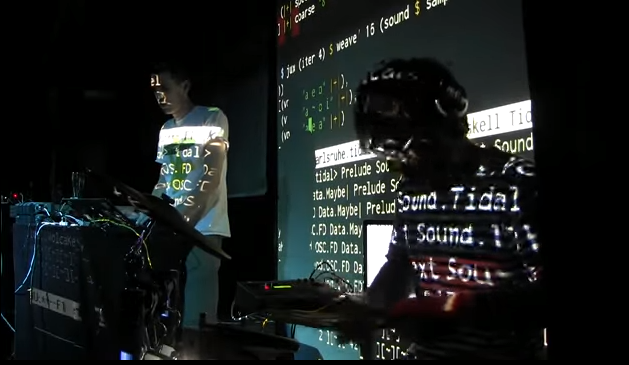
\includegraphics[scale=0.71]{imagens/canute.png}
%  \caption{Performance do duo Canute (Karlesruhe, 2015) \textbf{Fonte}: %\citeonline{mclean_canute_2015}.}
%  \label{fig:canute}
%\end{figure}

%O registro audiovisual do duo Canute, Matthew Yee-King (bateria eletrônica) e Alex McLean (\emph{laptop}), reforça o arquétipo comentado anteriormente (p.~\pageref{fig:weaving}). A recomendação ``Obscurantismo é perigoso, mostre-nos suas telas''\ver{sec:showusyourscreens} é seguida à risca. Categorizações musicais como \emph{club} e \emph{chordpunch} são mencionados na descrição do vídeo. É curioso notar que, em alguns momentos do vídeo, certas modificações nos códigos causam uma perturbação brusca em sistema de ritmos, percebido através do fluxo musical. Em alguns momentos Yee-King mantem o fluxo, mas em outros o instante musical codificado leva um curto período de tempo para ser sincronizado, o que leva Yee-King a se confundir, e por um breve instante, escutar o código e aí retornar à execução. Essa quebra no fluxo musical pode atrapalhar o fluxo de movimentos do corpo. No final deste capítulo, discutimos que este pode não ser \emph{a priori} um erro do instrumentista, mas sim um problema entre o não-esforço cênico de McLean e o esforço de Yee-King. Esta questão cênica será mencionada na \autoref{sec:showusyourscreens}.

%\begin{figure}[h]
%  \centering
%  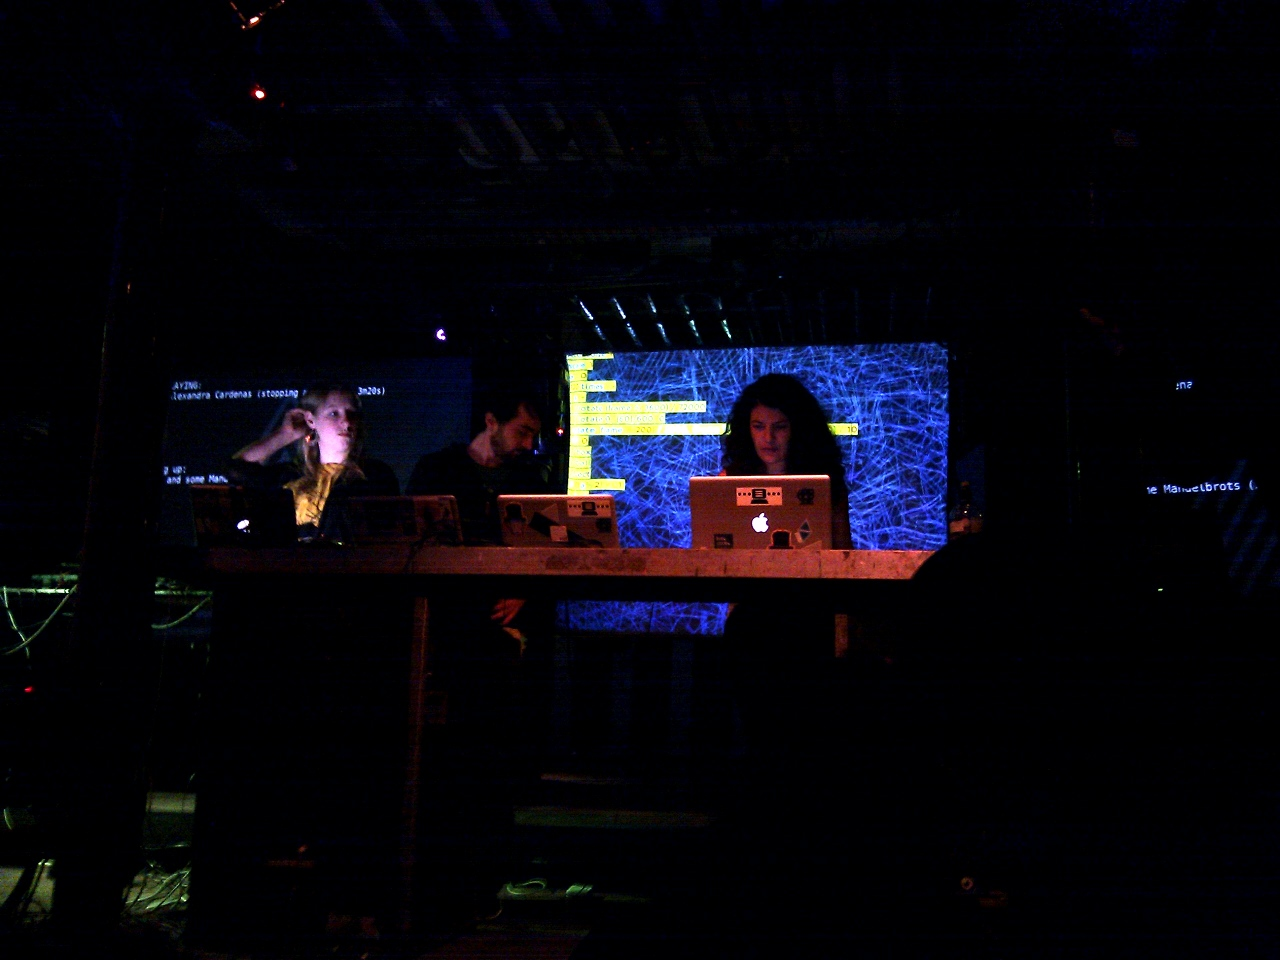
\includegraphics[scale=0.3]{imagens/cardenas.jpg}
%  \caption{Performance do duo Mico Rex (Londres, 2013) \textbf{Fonte}: %\citeonline{griffths_algorave_2013}.}
%  \label{fig:cardenas}
%\end{figure}

%\begin{figure}[!h]
%  \centering
%  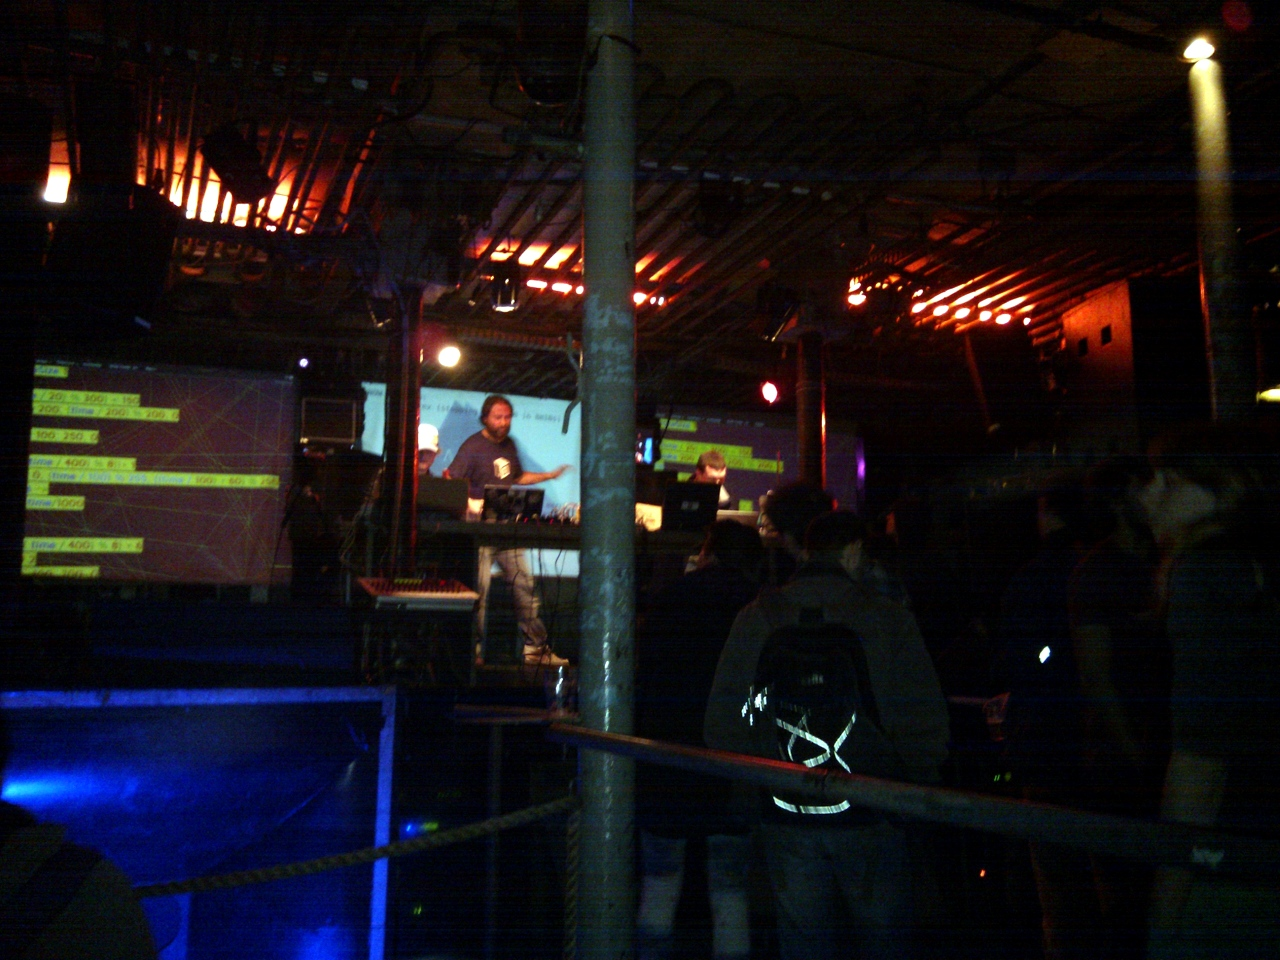
\includegraphics[scale=0.3]{imagens/algorave.jpg}
%  \caption{Performance do duo Mico Rex (Londres, 2013) \textbf{Fonte}: %\citeonline{griffths_algorave_2013}.}
%  \label{fig:micorex}
%\end{figure}

%Griffiths registra uma \emph{rave} na embarcação  MS Stubnitz, em Canary Wharf, Londres, em 2013. Cárdenas e Ernesto Romero/Jorge Ramírez -- Mico Rex, \ver{fig:micorex} -- tocam neste evento. Encontramos um registro audiovisual de curta duração da apresentação do duo Mico Rex\disponivelem{https://vimeo.com/65309754}, mas não de Cárdenas. Exemplos sonoros específicos estão disponíveis nas redes sociais \emph{SoundCloud} e \emph{Vimeo} \footnote{\url{https://soundcloud.com/tiemposdelruido} e \url{https://soundcloud.com/micorex/}.}. Notas descritivas nestes perfis especificam instrumentos e linguagens de programação, mas não o processo criativo. MicoRex utiliza voz e \emph{programação} ao vivo com o ambiente de programação \emph{SuperCollider}\ver{sec:supercollider}. Entre as categorizações musicais mencionadas, \emph{electro-pop}, \emph{8bits/glitch}, \emph{electro}, \emph{punk}, \emph{bolero} e \emph{breakz}. Cárdenas realiza suas performances com guitarra e programação ao vivo com o \emph{SuperCollider}. É interessante que Cárdenas menciona a utilização de\emph{techno}, \emph{dubstep} e \emph{noise} -- além de distorções, utliliza um misto de instrumento expandido (objetos diversos jogados, friccionados, apoiados na guitarra) e retroalimentação de sinais com níveis saturados.  

\section{Dança}\label{sec:coreografia}

Nesta seção contrapomos a visão da seção anterior através uma suíte coreográfica de Kate Sichio, \emph{Hacking the Body}. Discutimos a elaboração/codificação como parte de uma \emph{estratégia transversal} \footnote{\cfcite{Forth2010,McLean2011}}, de uma partitura de performances para um pseudo-código de computador, e finalmente em uma coreografia codificada ao vivo.

Para Sichio, a relação entre a atividade de escrever programas, e a Dança como composição de movimentos corporais, é parte de um trabalho contínuo entre notação de coreografias e a improvisação de movimentos. Este trabalho parte daquilo que \citeonline[p.~31]{sichio_hacking_2004}, através de \citeonline[cap.~1, p.~3]{downie_choreography_2005}, cita como \emph{Sensibilidades Computacionais}, ou dispositivos metafóricos elaborados por coreógrafos como Merce Cunningham, Trisha Brown, Bill T. Jones, e William Forsythe -- \traducao{``mecanismos de generalização e abstração, representação da coreografia e dança como computação}{mechanisms of generalization and abstraction, choreography as representation, dance as computation''} \cite[cap.~1, p.~2--4]{downie_choreography_2005}:

\begin{citacao}
\traducao{Esta sensibilidade computacional é presente em dois níveis nos trabalhos destes coreógrafos. Primeiramente, em seus processos coreográficos -- os sistemas, métodos, e notação, através dos quais os coreógrafos criam a dança. Segundo, no trabalho ele mesmo, finalizado, que aparece no palco e é interpretado pelo observador. -- \textbf{As primeiras invenções e proclamações de Cunningham $[$, como$]$ a democracia do espaço do palco, e a redescoberta do que está atrás do dançarino como ponto de origem do movimento -- podem ser interpretadas como generalizações do tipo}; qualquer ponto do palco é a ``frente'', e conectado por um conjunto de articulações pode ser pensado como um membro. O que eram constantes, uma vez especificados em uma descrição rígida, se tornam variáveis em uma estrutura generativa.}{This computational sensibility is present at two levels in the work of these choreographers. Firstly, in their choreographic processes — the systems, methods, and notations through which the choreographers create the dance. Secondly, in the finished work itself, as it appears on stage and as it is interpreted by the viewer. (\ldots) Cunningham’s earliest inventions and proclamations — the democracy of the stage space, and the rediscovery of the dancer’s back as a point of origin of motion — can be interpreted as generalizations of a kind; any point of a stage can be a “front”, and any connected set of joints can be thought of as a limb. What were once specified constants in a rigid description become variables in in a generative framework.\emph{Grifo nosso}.}
\end{citacao}

\subsection{Hacking Coreography}

A improvisação de códigos parte de uma proposição (\emph{v.01}): \emph{hackear} uma Partitura de Eventos do artista Alison Knowles (mais especificamente a peça de performance \#8, de 1965), e projetá-la em um espaço de performance, onde dançarinos lêem a partitura (ver exemplo \ref{code:knowles}), sem ensaios prévios: 

\begin{example}{Partitura original de Alison Knowles (1965)}\label{code:knowles}
\scriptsize
Divida uma variedade de objetos em dois grupos. 
Cada grupo é rotulado com "tudo". 
Estes grupos podem incluir diversas pessoas. 
Existe uma terceira divisão do palco, objetos vazios, rotulados com "nada". 
Cada um dos objetos é "alguma coisa". 
Um executante combina e ativa os objetos das seguintes maneiras para qualquer duração desejada de tempo :

• "alguma coisa" com "tudo"

• "alguma coisa" com "nada"

• "alguma coisa" com "alguma coisa"

• "tudo" com "tudo"

• "tudo" com "nada"

• "nada" com "nada"
\end{example}

A orientação (\emph{hack}) de Knowles aos dançarinos é que executem a partitura original integralmente uma única vez. No momento em que a última rotina de movimentos (combinar "nada" com "nada"), deve ocorrer uma desconstrução dos rótulos originais através de separações de suas sílabas , de forma que são derivados novos rótulos para novas recombinações:

\begin{citacao}
\traducao{Depois que a partitura foi completada, contudo, ela foi \emph{hackeada}. Isso significa que o executante tenta de alguma forma contornar as instruções originais. Isto foi feito sem preparações prévias e a audiência assistiu isso se desdobrar enquanto era realizada. Nesta primeira performance, o papel e os rótulos foram rasgados para criar novas palavras e categorias (\ldots) Então ao invés de ``nada''$[$Nothing$]$, foram formados dois grupos, ``não''$[$No$]$ e ``coisa''$[$Thing$]$.}{After the score was completed, however, it was then hacked. This meant that the performer had to try to somehow circumvent the original instructions. This was done with no previous preparation and the audience watched this unfold as the piece was performed.In this first performance, the paper and the labels were torn up to create new words and categories (\ldots). So instead of “Nothing” there were two new groups, “No” and “Thing.”}
\end{citacao}

A segunda experiência, \emph{Hacking Coreography beta v.02}, é inspirada na mesma partitura de Alison Knowles, agora com o objetivo de definir algoritmos associados a um termo técnico de movimento corporal, híbridos de texto discursivo e código de computador em linguagem Java. Isto é, o código é executável por um computador para resultar em sons ou imagens, mas por um humano para resultar em movimentos.

\begin{example}{Exemplo de um hackeamento de partitura de movimentos}
\begin{minted}[fontsize=\scriptsize]{java}
/Dance/
set up()
{
dance a centre, right
dance b centre, left
}

movement()
{
move1 (dance a = rotate) (dance b = jump)
move2 (dance a = brush) (dance b = lie down)
move3 (dance a = push) (dance b = run)
move4 (dance a = step) (dance b = kneel)
}

coreography()
{
if (dancer a = rotate right 180)
then both jump = 2 feet to 1
if (dancer b = travels)
then brush = right foot
}

run(){
move1
move4
move4
move1
move2
move3
move1
move2
move3
move4
}

/hack/
{
if (dancer a = kneel)
dancer a = kneel
if (dancer a = rotate)
dancer b = rotate opposite direction 
}
\end{minted}
\end{example}

Algumas seções são apresentadas como \emph{funções} (\emph{set up, movement, coreography \emph{e} run}). A função \emph{set up} define as posições iniciais de cada ator; \emph{movement} define os tipos de movimentos que serão executados por intérpretes; \emph{coreography} define uma estrutura de fluxo destes movimentos; e por último, uma ordem de execuções é estruturada em \emph{run}. É interessante notar que Sichio aponta para um outro \emph{hackeamento} da partitura. A utilização de números, como por exemplo na função \emph{coreography}, dificultou a leitura dos intérpretes durante ensaios. Uma alteração na função \emph{coreography}, notificada abaixo da linha \verb|/hack/|, foi feita pelos próprios intérpretes para alterar a notação numérica por uma descrição textual da ação. Isso tornou o código mais legível para humanos durante a execução de movimentos. 

\subsection{Hacking the Body}

O \emph{Hacking The Body 2.0}, ou \emph{HTB2.0} (2015)\disponivelem{https://www.youtube.com/watch?v=iOAffWTBVE0} é uma performance posterior de Sichio, que seguiu desenvolvimentos posteriores aos citados na seção anterior.

A coreógrafa está sentada em uma penumbra. Já uma dançarina recebe aos poucos uma iluminação contrastante, com uma vestimenta branca e uma iluminação frontal \ver{fig:iclcdanca}. A coreógrafa improvisa um código de movimentos corporais que são executados por outra mulher:

\begin{citacao}
\traducao{Esta peça é uma exploração de eletrônica codificada ao vivo e movimentos improvisados. Uma dançarina veste uma peça de atuadores hápticos. Estes atuadores são programados em tempo-real via OSC\footnote{N.A.: ``\emph{Open Sound Control} é um protocolo de comunicação entre computadores, sintetizadores sonoros e outros dispositivos multimídia que são otimizados para as modernas tecnologias de rede''. Disponível em \url{http://opensoundcontrol.org/introduction-osc}} para 'zunir' sobre os lados direito e esquerdo da dançarina para indicar qual lado do corpo a dançarina deve mover. A partitura é codificada ao vivo pela coreógrafa enquanto a dançarina responde por uma retroalimentação háptica. Esta peça explora o \emph{live coding} de corpos, e movimento como saída, ao invés de saídas sonoras ou visuais como encontrado em muitas execuções de \emph{live coding}
}{
This dance piece is an exploration of live coded electronics and improvisational movement. A dancer wears a custom garment of haptic actuators. These actuators are programmed real-time via OSC to 'buzz' on the right and left sides of the dancer to indicate which side of the body the dancer will move. The score is being live coded by choreographer while the dancer is responding to the haptic feedback. This piece explores live coding of bodies and movement as output rather than a sonic or visual output as found in many live coding performances. \emph{Disponivel em \url{http://iclc.livecodenetwork.org/performances.html}}.
}
\end{citacao}

\begin{figure}[!h]
 \centering
  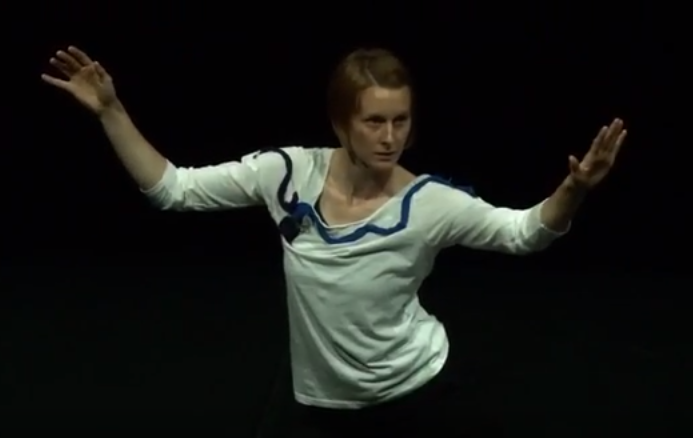
\includegraphics[scale=0.6]{imagens/iclcdanca.png}
  \caption{Dançarina (anônima) controlada por Kate Sicchio (2015) através de uma codificação improvisada. \textbf{Fonte}: \url{https://www.youtube.com/watch?v=uAq4BAbvRS4}.}
  \label{fig:iclcdanca}
\end{figure}

Como aponta a própria coreógrafa, a maioria das performances de improviso de códigos segue o seguinte procedimento: o código é criado, e um som, uma nota, uma imagem ou um vídeo são gerados, combinados, transformados de maneira contínua. Mas o padrão é a realização audiovisual. Mesmo em algumas performances de dança pesquisadas (e que não foram mencionadas neste documento), a dança e a projeção audiovisual se suportam. A criatividade deste trabalho toca na seguinte pergunta: qual é o \emph{dispositivo de entrada e de saída} praticado nas improvisações de códigos? Sicchio responde que o corpo já é um dispositivo de entrada e saída de interações sociais e pode ser controlado por outro humano através de comandos de rede. A sensação de quietude existe não por questões musicais, mas por perguntar por onde passam os fluxos de informações digitais.

\section{Discussão}

Neste capítulo, delimitamo-nos a exemplificar ciclos de elaboração e codificação de uma proposição artística. De acordo com o antropólogo Giovanni Mori, esta proposição artística pode ser musical, visual, coreográfica ou têxtil. Afim de ilustrar a pluralidade da técnica de improvisação, escolhemos descrever duas formas, a têxtil e a coreográfica. O Audiovisual foi descrito como uma abordagem satélite, o que certamente encoraja futuras pesquisas na área específica.  A Música não ganhou foco neste capítulo, de forma que será destacada nos próximos dois capítulos. No \autoref{cap:protohistoria} (ver p.~\pageref{cap:protohistoria}), situamos propostas prototípicas de uma improvisação musical realizada através de computadores, nos moldes do \emph{live coding}. No \autoref{cap:estudos_de_caso} (ver \pageref{cap:estudos_de_caso}), analisaremos uma proposta, seu primeiro ciclo de elaboração e codificação em código de linguagem LISP, e um simples resultado sonoro.
